\documentclass[a4paper,11pt]{report}
\usepackage[utf8]{vietnam}
\usepackage[utf8]{inputenc}
\usepackage[dvipsnames,svgnames,table]{xcolor}
\usepackage{graphicx}
\usepackage{multirow}
\usepackage{multicol}
\usepackage{fancybox}
\usepackage{xcolor}
\definecolor{dkgreen}{rgb}{0,0.6,0}
\definecolor{gray}{rgb}{0.5,0.5,0.5}
\definecolor{mauve}{rgb}{0.58,0,0.82}
\definecolor{hilight}{RGB}{22,155,104}
  
\definecolor{Xanh}{rgb}{0,0.5,1}
\definecolor{Do}{rgb}{1,0.25,0}
\definecolor{Vang}{rgb}{1,1,0}
\definecolor{Datroi}{rgb}{0,0,1}
\usepackage{listings}
\usepackage{amsmath}
\usepackage{amssymb}
\usepackage[linesnumbered,ruled]{algorithm2e}
\usepackage[colorlinks = true,
            linkcolor = black,
            urlcolor  = blue,
            citecolor = blue,
            anchorcolor = blue]{hyperref}
\usepackage{longtable}
\usepackage{listings}
\newcommand{\bi}{\begin{itemize}}
\newcommand{\ei}{\end{itemize}}
\lstset{language=C++,
   %keywords={break,case,catch,continue,else,elseif,end,for,function,
   %   global,if,otherwise,persistent,return,switch,try,while},
   basicstyle=\ttfamily \fontsize{10}{12}\selectfont,   
   numbers=left,
   frame=lrtb
  }

\usepackage[left=3cm, right=2.00cm, top=2.00cm, bottom=2.00cm]{geometry}
\begin{document}
\thispagestyle{empty}
\thisfancypage{
\setlength{\fboxrule}{1pt}
\doublebox}{}
\begin{center}
{\fontsize{16}{19}\fontfamily{cmr}\selectfont TRƯỜNG ĐẠI HỌC BÁCH KHOA HÀ NỘI\\
VIỆN CÔNG NGHỆ THÔNG TIN VÀ TRUYỀN THÔNG}\\
\textbf{------------*******---------------}\\[1cm]

\includegraphics[scale=0.13]{hust.jpg}\\[1.3cm]

{\fontsize{32}{43}\fontfamily{cmr}\selectfont BÁO CÁO}\\[0.1cm]
{\fontsize{38}{45}\fontfamily{cmr}\fontseries{b}\selectfont MÔN HỌC}\\[0.2cm]
{\fontsize{19}{20}\fontfamily{phv}\selectfont Khai phá dữ liệu}\\[1cm]
{\fontsize{17}{24}\fontfamily{cmr}\selectfont Đề tài:}\\[1cm]
{\fontsize{17}{24}\fontfamily{cmr}\selectfont Phân loại tin nhắn SMS}\\[1.5cm]
\end{center}
\hspace{1cm}\fontsize{14}{16}\fontfamily{cmr}\selectfont \textbf{Sinh viên thực hiện:}
\begin{longtable}{l c c }
Họ và Tên & MSSV &    Mã học phần \\[0.5cm]
Đặng Quang Trung &    20134145 & IT4768\\
Trịnh Văn Duy & 20130614 & IT4768 \\
Trần Văn Thành & 20133561 & IT4768 \\
\end{longtable}
\hspace{0.3cm}\fontsize{14}{16}\fontfamily{cmr}\selectfont \textbf{Giáo viên hướng dẫn:} TS. Trịnh Anh Phúc\\[1.0cm]
\begin{center}
\fontsize{16}{19}\fontfamily{cmr}\selectfont Hà Nội 14-05-2017
\end{center} 
\tableofcontents
%\chapter*{Lời mở đầu}
%\addcontentsline{toc}{chapter}{Lời mở đầu}
%Sự phát triển của công nghệ thông tin và việc ứng dụng công nghệ thông tin trong nhiều
%lĩnh vực của đời sống, kinh tế xã hội trong nhiều năm qua cũng đồng nghĩa với lượng dữ
%liệu đã được các cơ quan thu thập và lưu trữ ngày một tích luỹ nhiều lên. Họ lưu trữ các
%dữ liệu này vì cho rằng trong nó ẩn chứa những giá trị nhất định nào đó. Mặt khác, trong
%môi trường cạnh tranh, người ta ngày càng cần có nhiều thông tin với tốc độ nhanh để trợ
%giúp việc ra quyết định và ngày càng có nhiều câu hỏi mang tính chất định tính cần phải
%trả lời dựa trên một khối lượng dữ liệu khổng lồ đã có. Với những lý do như vậy, các
%phương pháp quản trị và khai thác cơ sở dữ liệu truyền thống ngày càng không đáp ứng
%được thực tế đã làm phát triển một khuynh hướng kỹ thuật mới đó là Kỹ thuật phát hiện
%tri thức và khai phá dữ liệu. \\ \\ 
%Khai phá dữ liệu đã và đang được nghiên cứu, ứng dụng trong nhiều lĩnh vực khác nhau
%ở các nước trên thế giới, tại Việt Nam kỹ thuật này tương đối còn mới mẻ tuy nhiên cũng
%đang được nghiên cứu và dần đưa vào ứng dụng. Khai phá dữ liệu là một bước trong qui
%trình phát hiện tri thức gồm có các thuật toán khai thác dữ liệu chuyên dùng dưới một số
%qui định về hiệu quả tính toán chấp nhận được để tìm ra các mẫu hoặc các mô hình trong
%dữ liệu. Nói một cách khác, mục đích của phát hiện tri thức và khai phá dữ liệu chính là
%tìm ra các mẫu và/hoặc các mô hình đang tồn tại trong các cơ sở dữ liệu nhưng vẫn còn bị
%che khuất bởi hàng núi dữ liệu. \\ \\ 
%Trong bài viết này, em sẽ trình bày một cách tổng quan về Kỹ thuật khai phá dữ liệu.
%Trên cơ sở đó đưa ra một bài toán lọc thư rác cho người dùng của một hệ thống và giải quyết bài toán bằng phương pháp naivebayes và svm.

\chapter*{Lời cảm ơn}
\addcontentsline{toc}{chapter}{Lời cảm ơn}
Chúng em xin chân thành cảm ơn thầy Trịnh Anh Phúc đã cung cấp cho chúng em những kiến thức vô cứng bổ ích khi chúng em bắt đầu tìm hiểu về môn học khai phá dữ liệu cũng như đã giúp đỡ chúng em rất nhiều trong quá trình thực nghiệm và viết bản báo cáo này.
\chapter{Mô tả bài toán}
Bài toán yêu cầu phân loại các tin nhắn chưa được gán nhãn thành 2 loại là tin nhắn rác (spam) và tin nhắn thông thường (ham). Dữ liệu cho là 100 tin nhắn đã được gán nhãn ( 1 tương ứng với ham và -1 tương ứng với spam). Đây là một bài toán Khai phá dữ liêu ( Học máy) trên text với đặc điểm là tin nhắn tương đối ngắn, chứa nhiều ký tự đặc biệt, cần xử lý tốt trước khi tiến hành phân loại.
\chapter{NaiveBayes}
\section{Xử lý dữ liệu}
\begin{itemize}
\item[•] Lower hóa tất cả cách word sau khi được tiền xử lý ở hai bước trên.
\item[•] Loại bỏ các kí tự gây nhiễu như: [](),"
\item[•] Tách các mẫu tin thành các term n-gram (n = 3).
\item[•] Xây dựng bộ từ điển theo các term sau khi phân tách n-gram.
\end{itemize}
\section{Mô hình naivebayes}
\subsection{Định lí naivebayes}
\begin{displaymath}
P(h|D) = \frac{P(D|h).P(h)}{P(D)}
\end{displaymath} 
\begin{itemize}
\item[•] P(h): Xác suất trước (tiên nghiệm) của giả thiết (phân loại) h
\item[•] P(D): Xác suất trước (tiên nghiệm) của việc quan sát được
dữ liệu D
\item[•] P(D|h): Xác suất (có điều kiện) của việc quan sát được dữ
liệu D, nếu biết giả thiết (phân loại) h là đúng
\item[•] P(h|D): Xác suất (có điều kiện) của giả thiết (phân loại) h là đúng, nếu quan sát được dữ liệu D
\end{itemize}
\subsection{NaiveBayes cho phân loại spam}
Cho một tài liệu d(ở đây là một tin nhắn văn bản sms) và một nhãn c(nhẵn c nhận giá trị 1 và - 1 tương ứng với ham và spam).Ta có xác suất để d được phân vào nhãn c theo công thức:
\begin{displaymath}
P(c|d) = \frac{P(d|c).P(c)}{P(d)}
\end{displaymath}
Ta sẽ gắn cho d một nhẵn lớp có khả năng nhất theo:
\begin{displaymath}
\displaystyle c_{MAP} = \arg\max_{c\in C} P(c|d) = \arg\max_{c\in C} \frac{P(d|c)P(c)}{P(d)} = \arg\max_{c\in C} P(d|c)P(c)
\end{displaymath}
Xác suất P(d) là như nhau với mọi tin nhắn d. \\
Tin nhắn d được biểu diễn bởi 1 số thuộc tính nên ta có công thức:
\begin{displaymath}
\displaystyle c_{MAP} = \arg\max_{c\in C} P(d|c)P(c) = \arg\max_{c\in C} P(x_1,x_2,\ldots,x_n|c)P(c)
\end{displaymath}
Trong đó:
\begin{itemize}
\item[•] $x_1, x_2,\ldots, x_n$ là vector các thuộc tính biểu diễn tin nhắn.
\end{itemize}
Các thuộc tính là độc lập với nhau nên ta có:
\begin{displaymath}
\displaystyle c_{NB} = \arg\max_{c\in C}P(c_j)\Pi_{x\in X}P(x|c)
\end{displaymath}
Một tin nhắc sẽ được biểu diễn bởi 1 số các thuộc tính nên xác suất phân nhãn cho một tin nhắn:
\begin{displaymath}
\displaystyle c_{NB} = \arg\max_{c_j\in C}P(c_j)\Pi_{x_i \in X_d}P(x_i|c)
\end{displaymath}
Trong đó:
\begin{itemize}
\item[•] $X_d$ là tập thuộc tính biểu diễn tin nhắn d.
\item[•] $c_j$ tương ứng với nhẵn j trong danh sách nhẵn.
\end{itemize}
\subsection{Ước lượng maximum likelihood}
\begin{displaymath}
\displaystyle
\hat{P}_{c_j} = \frac{doccount( C = c_j)}{N_{doc}}
\end{displaymath}
\begin{displaymath}
\displaystyle
\hat{P}_{w_i|c_j} = \frac{count(w_i,c_j)}{\sum_{w\in V} count(w,c_j)}
\end{displaymath}
Trong đó:
\begin{itemize}
\item[•] $doccount(C = c_j)$ số tin nhắn có nhãn ứng với $c_j$.
\item[•] $count(w_i,c_j)$ số lần xuất hiện $w_i$(một term, word hay thuộc tính) trong các tin nhắn có nhẵn tương ứng là $c_j$.
\end{itemize}
Vấn đề $\hat{P}_{w_i|c_j} = \frac{count(w_i,c_j)}{\sum_{w\in V} count(w,c_j)} = 0$ nếu $w_i$ không có trong tập train dẫn đến dự đoán sai. \\
Để khăc phục điều này và làm naive bayes mượt hơn dùng công thức sau thay thế:
\begin{displaymath}
\displaystyle
\hat{P}_{(w_i|c)} = \frac{count(w_i,c) + 1}{\sum_{w\in V}(count(w,c) + 1)} = \frac{count(w_i,c) + 1}{\sum_{w\in V}(count(w,c)) + |V|}
\end{displaymath}
\section{Phân phối gaussian}
\begin{itemize}
\item[•] Dữ liệu thuộc vào 2 lớp đã biết là Ham và Spam. Mỗi lớp đều có phân bố độ dài tin nhắn normal với trung bình và độ lệch chuẩn $\mu_{spam}$ và $\sigma_{spam}$ cho phân lớp spam và $\mu_{ham}$ và $\sigma_{ham}$ cho phân lớp ham
\item[•] Chúng ta có thể định nghĩa một mô hình bằng cách lấy mẫu từ các phân bố này, sử dụng phân lớp Spam với xác suất $P_{spam}$ và phân lớp B với xác suất $P_{ham}$ (trong đó $P_{spam}$ + $P_{ham}$ = 1)
\end{itemize}
Các chuẩn được tính theo công thức với $n = n_{spam}$ hoặc $n = n_{ham}$.
\begin{displaymath}
\mu = \frac{X_1 + X_2 + X_3 + X_4 + \ldots + X_{n-1} +X_n}{n}
\end{displaymath}
\begin{displaymath}
\sigma^2 = \frac{(X_1 - \mu)^2 + (X_2 - \mu)^2 + \ldots + (X_n - \mu)^2}{n - 1}
\end{displaymath}
Cho một tin nhắc sms $x_i$ xác suất để thuộc phân lớp là A là spam hoăc ham là:
\begin{displaymath}
\displaystyle
P(A|x_i) = \frac{P(x_i|A).P(A)}{P(x_i)} = \frac{N(x_i,\mu_A ,\sigma_A )P_A}{N(x_i,\mu_A ,\sigma_A )P_A + N(x_i,\mu_B ,\sigma_B )P_B}
\end{displaymath}
Ở đây N() là chuẩn của phân phối Gaussian công thức của N():
\begin{displaymath}
N(X,\mu ,\sigma ) = \frac{1}{\sqrt{2\pi}\sigma}e^{-\frac{(X - \mu)^2}{2\sigma^2}}
\end{displaymath}
\subsection{Công thức dư đoán}
\begin{displaymath}
\displaystyle c_{NB} = \arg\max_{c_j\in C}P(c_j)P(c_j|len(d))\Pi_{x_i \in X_d}P(x_i|c_j)
\end{displaymath}
\chapter{Logistic}
\section{Giới thiệu TF-IDF}
TF-IDF (Term Frequency-Inverse Document Frequency) là 1 kĩ thuật khai phá dữ liệu từ text sử dụng để phân loại văn bản . Trọng số này sử dụng để đánh giá tầm quan trọng của một từ trong một văn bản , 1 collection hoặc một corpus . Độ quan trọng tăng dần dựa vào số lần từ xuất hiện trong văn bản nhưng bù lại bởi tần suất của từ đó trong corpus . Một vài biến thể của tf-idf thường xuyên được sử dụng trong các hệ thống tìm kiếm như một công cụ chính để đánh giá và sắp xếp văn bản dựa vào user query. Tf-idf có thể sử dụng để lọc những từ stop-words trong một số bài toán như tóm tắt văn bản và phân loại văn bản . \\ \\
\textbf{TF : Term Frequency} , là số lần term xuất hiện trong văn bản . Vì các văn bản có thể có độ dài ngắn khác nhau nên mọt số term có thể xuất hiện nhiều lần trong một văn bản dài hơn là một văn bản ngắn . Như thế , term frequency thường được chia cho độ dài văn bản ( tổng số term trong một văn bản) như một các normalization . \\ \\
\textbf{IDF: Inverse Document Frequency}, đánh giá tầm quan trọng của một term . Khi tính toán TF , tất cả các terms được coi như có độ quan trọng như nhau . Nhưng một số terms, như “is” , “of” và “that” thường xuất hiện rất nhiều lần nhưng độ quan trọng là không cao . Như thế chúng ta cần giảm wegh xuống \\ \\
IDF(t) = log(Tổng số văn bản/ Số văn bản chứa term t ). \\  \\
Ví dụ một văn bản chưa 100 từ mà từ “cat” xuất hiện 3 lần . Term frequency cho từ cat này là (3/100) = 0.03 . Giả sử , chúng ta có 10 triệu văn bản và từ “cat” xuất hiện trong một nghìn văn bản . Như thế , idf được dính là log(10,000,000 / 1,000) = 4. Như thế , tf-idf của từ “cat” trong văn bản này sẽ là : 0.03 * 4 = 0.12. \\
\section{Giới thiệu về phân loại Logistic regression}
Là một bộ phân loại với khá mạnh mẽ, có thể áp dụng cho những bài toán phân loại phi tuyến, phù hợp với trường hợp dữ liệu để huấn luyện ít, trong bài toán của chúng ta, bộ phân loại này là thích hợp cùng với bộ phân loại văn bản Naive Bayes
Hàm dự đoán của bộ phân loại này có dạng:
\begin{displaymath}
h_{\theta}(x) = g(\theta^T x)
\end{displaymath}
\begin{displaymath}
g(z) = \frac{1}{1 + e^{-z}}
\end{displaymath}
Trong đó:
\begin{itemize}
\item[-] $\theta$ là trọng số tương ứng với đặc trưng dữ liệu x-i.
\item[-] Hàm g(z) ở đây được gọi là hàm sigmoid hay hàm logistic.
\end{itemize}
Áp dụng với bài toán của chúng ta, bộ phân loại sẽ phân loại tin nhắn là spam nếu $h_{\theta}(x) \geq 0.5$ và sẽ phân loại tin nhắn là ham nếu ngược lại. Đồ thị của hàm phân loại có dạng:
\begin{figure}[h]
\begin{center}
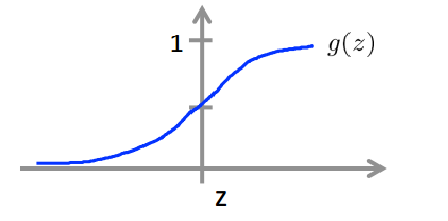
\includegraphics[scale=0.8]{gz.png}
\caption{Hình minh họa hàm g(z)}
\end{center}
\end{figure}
\\
Hàm mất mát (loss function) được định nghĩa theo công thức:
\begin{displaymath}
\displaystyle
J(\theta) = \frac{1}{m}\sum_{i=1}^{m}[-y^{(i)}log(h_\theta(x^{(i)})) - (1 - y^{(i)})log(1 - h_\theta x^{(i)}))]
\end{displaymath}
Hàm này sẽ được tối ưu theo thuật toán gradient decent hay bất kỳ thuật toán tối ưu không ràng buộc nào khác. Đối với bài toán của chúng ta, sau khi vector hóa tin nhắn bằng trọng số TF-IDF, ta sẽ fit dữ liệu vào bộ phân loại này, kết quả tốt hơn so với khi sử dụng SVM, bởi vì dữ liệu huấn luyện ở đây tương đối ít.
\section{Tiền xử lý}
\begin{itemize}
\item[•] Mã hóa các xâu có pattern phù hợp, ví dụ các từ trong tin nhắn khớp với pattern date sẽ được thay thế bằng từ 'date', các từ khớp với phone\_pattern sẽ được thay thế bằng từ 'phone', tương tự với link\_pattern, currency\_pattern, emotion\_pattern, number\_pattern và sex\_pattern. Quá trình này được thực hiện trên cả tập Train và Test.
\item[•] Thay thế các ký tự đặc biệt, quan trọng, giữ lại dấu ? và thay thế bằng 'qMark', còn lại các ký tự đặc biệt khác không khớp với pattern\_emotion sẽ được thay thế bằng dấu cách.
\item[•] Lower hóa tất cả cách word sau khi được tiền xử lý ở hai bước trên
\item[•] Với những bước tiền xử lý trên, ta sẽ dùng bộ đánh trọng số TF-IDF với những tin nhắn trong tập train, cùng với đó là fit bộ đánh trong số đó cho tập test.
\end{itemize}
\section{Quá trình trainning}
\begin{itemize}
\item[•] Dữ liệu gồm 100 tin nhắn sau khi được tiền xử lý
\item[•] Sẽ được chia thành tập train gồm 75 tin nhắn, tập validate để tuning tham số gồm 25 tin nhắn còn lại.
\item[•] Kết quả được đánh giá dựa trên các ước lượng % độ chính xác, recall, precision và cuối cùng là điểm F1
\item[•] Sử dụng bộ phân loại Logistic Regression ( Vì bộ phân loại này thích hợp hơn so với SVM do tập train quá ít dữ liệu)
\item[•] Kết quả tương đối tốt ( F1= 0.85 -> 0.97) 
\end{itemize}
\section{Quá trình Test với bộ dữ liệu của Thầy}
\begin{itemize}
\item[•] Sử dụng toàn bộ 100 tin nhắn để train như trước
\item[•] Và chạy test trên 300 tin nhắn thầy gửi.
\end{itemize}
Sau đây là code python (3.5) thể hiện ý tưởng trên. Để chạy được code này cần cài đặt các thư viện numpy, sklearn, và codecs. Các file test.txt và train.txt được đặt ở cùng một thư mục với file source code.
\begin{lstlisting}
import numpy as np
import re 
from sklearn.linear_model.logistic import LogisticRegression
from sklearn.cross_validation import train_test_split, cross_val_score
from sklearn.feature_extraction.text import TfidfVectorizer
from sklearn.metrics import accuracy_score
from sklearn.metrics import confusion_matrix
from builtins import str
import codecs
date_pattern = []
phone_pattern = []
link_pattern = []
currency_pattern = []
emotion_pattern = []
number_pattern=[]
sex_pattern=[]

date_string = ' date '
phone_string = ' phone '
link_string = ' link '
currency_string = ' currency '
emotion_string = ' emotion '
number_string=' number '
sex_string=' sex'

date_pattern.append(r'\d{1,2}/\d{1,2}/\d{2,4}')
date_pattern.append(r'\d{1,2}-\d{1,2}-\d{2,4}')
date_pattern.append(r'\+\d{1,2}:\d{1,4}')
date_pattern.append(r'\d{1,2}/\d{1,4}')
date_pattern.append(r'\d{1,2}-\d{1,4}')
date_pattern.append(r'\d{1,2}h\d{0,2}')
date_pattern.append(r'phut')
date_pattern.append(r'giay')

phone_pattern.append(r'\+\d{10,12}')
phone_pattern.append(r'\d{3,5}\.\d{3,4}\.\d{3,5}')
phone_pattern.append(r'\d{8,12}')
phone_pattern.append(r'1800\d{2,4}')
phone_pattern.append(r'1900\d{2,4}')
phone_pattern.append(r'\d{4}')
phone_pattern.append(r'[0]\d{2,3}')
phone_pattern.append(r'195')
phone_pattern.append(r'900')
phone_pattern.append(r'999')
phone_pattern.append(r'1342')
phone_pattern.append(r'191')
phone_pattern.append(r'888')
phone_pattern.append(r'333')
phone_pattern.append(r'1414')
phone_pattern.append(r'1576')
phone_pattern.append(r'8170')
phone_pattern.append(r'9123')
phone_pattern.append(r'9118')
phone_pattern.append(r'266')
phone_pattern.append(r'153')
phone_pattern.append(r'199')
phone_pattern.append(r'9029')
phone_pattern.append(r'8049')
phone_pattern.append(r'1560')
phone_pattern.append(r'9191')
phone_pattern.append(r'8709')
phone_pattern.append(r'9241')
phone_pattern.append(r'7393')
phone_pattern.append(r'7719')

link_pattern.append(r'www\..*')
link_pattern.append(r'http://.*')

currency_pattern.append(r'[0-9|\,\.]{3,}VND')
currency_pattern.append(r'[0-9|\.]{3,}VND')
currency_pattern.append(r'[0-9|\.]{3,}d')
currency_pattern.append(r'[0-9|\.]{3,}d')
currency_pattern.append(r'[0-9|\.]{3,}tr')
currency_pattern.append(r'[0-9|\.]{3,}Tr')
currency_pattern.append(r'[0-9|\.]{3,}TR')
currency_pattern.append(r'\d{1,3}trieu')
currency_pattern.append(r'\d{1,3}tr')
currency_pattern.append(r'\d{1,1000}ti')
currency_pattern.append(r'\d{1,3}k')
currency_pattern.append(r'\d{1,3}nghin')
currency_pattern.append(r'\d{1,3}tram')

emotion_pattern.append(r'o.O')
emotion_pattern.append(r'O.o')
emotion_pattern.append(r'\(y\)')
emotion_pattern.append(r'\(Y\)')
emotion_pattern.append(r':v')
emotion_pattern.append(r':V')
emotion_pattern.append(r':3')
emotion_pattern.append(r'-_-')
emotion_pattern.append(r'\^_\^')
emotion_pattern.append(r'<3')
emotion_pattern.append(r':-\*')
emotion_pattern.append(r':\*')
emotion_pattern.append(r":'\(")
emotion_pattern.append(r':p ')
emotion_pattern.append(r':P')
emotion_pattern.append(r':d')
emotion_pattern.append(r':D')
emotion_pattern.append(r':-\?')
emotion_pattern.append(r'>\.<')
emotion_pattern.append(r'><')
emotion_pattern.append(r':-\w ')
emotion_pattern.append(r':\)\)')
emotion_pattern.append(r';\)\)')
emotion_pattern.append(r'=\)\)')
emotion_pattern.append(r':-\)')
emotion_pattern.append(r':\)')
emotion_pattern.append(r':\]')
emotion_pattern.append(r'=\)')
emotion_pattern.append(r':-\(')
emotion_pattern.append(r':\(')
emotion_pattern.append(r':\[')
emotion_pattern.append(r'=\(') 
emotion_pattern.append(r'sock')
emotion_pattern.append(r'haizz')
    
  
sex_pattern.append(r'xxx')  
sex_pattern.append(r'sexy')  
sex_pattern.append(r'9x')
  
number_pattern.append(r'\d{1,}')
corpus=list()
labels=list()
test_corpus=list()
test_corpus_to_print=list()
file_train=codecs.open('train.txt','r','utf-8')
file_test=codecs.open('test.txt','r')
for line in file_train:
    if line[0]=='1':
        labels.append(1)
        corpus.append(line[1:].strip().lower())
    else:
        labels.append(-1)
        corpus.append(line[2:].strip().lower())

for line in file_test:
    test_corpus.append(line[1:].strip().lower())
    test_corpus_to_print.append(line[1:].strip())


# test_corpus_to_print=test_corpus

i=0
for line in corpus:
    for pattern in date_pattern:
        line=re.sub(pattern, date_string, line)
    for pattern in emotion_pattern:
        line=re.sub(pattern, emotion_string, line)
    for pattern in sex_pattern:
        line=re.sub(pattern, sex_string, line)    
    for pattern in currency_pattern:
        line=re.sub(pattern, currency_string, line)
    for pattern in phone_pattern:
        line=re.sub(pattern, phone_string, line)
    for pattern in link_pattern:
        line=re.sub(pattern, link_string, line)
    for pattern in number_pattern:
        line=re.sub(pattern, number_string, line)
    line=line.replace('?',' qMark ')
    line=line.replace('$',' currency ')
    stop_list = ['.', ',', '/', ';', ':', '&', '@', '!', '`',
               "'", '"', '>', '<', '*', '%', '#', '(', ')', '[',']',
              '-', '_', '=', '+', '{', '}', '~', '^', '*', '|', '\\']
    for item in stop_list:
        line=line.replace(item,' ')
    corpus[i]=line
    i+=1



i=0
for line in test_corpus:
    for pattern in date_pattern:
        line=re.sub(pattern, date_string, line)
    for pattern in emotion_pattern:
        line=re.sub(pattern, emotion_string, line)
    for pattern in sex_pattern:
        line=re.sub(pattern, sex_string, line)
    for pattern in currency_pattern:
        line=re.sub(pattern, currency_string, line)
    for pattern in phone_pattern:
        line=re.sub(pattern, phone_string, line)
    for pattern in link_pattern:
        line=re.sub(pattern, link_string, line)
    for pattern in number_pattern:
        line=re.sub(pattern, number_string, line)
    line=line.replace('?',' qMark ')
    line=line.replace('$',' currency ')
    stop_list = ['.', ',', '/', ';', ':', '&', '@', '!', '`',
    "'", '"', '>', '<', '*', '%', '#', '(', ')', '[',
     ']', '-', '_', '=', '+', '{', '}', '~', '^', '*', '|', '\\']
    for item in stop_list:
        line=line.replace(item,' ')
    test_corpus[i]=line
    i+=1



Vectorizer=TfidfVectorizer()
X_train_raw=corpus
y_train=labels
X_test_raw=test_corpus

# for i,item in enumerate(X_train_raw):
#     print(str(i)+" "+item)
X_train=Vectorizer.fit_transform(X_train_raw)
X_test=Vectorizer.transform(X_test_raw)
classifier=LogisticRegression()
classifier.fit(X_train, y_train)
predictions=classifier.predict(X_test)

for i in range(len(predictions)):
    print(str(predictions[i]) +" "+ test_corpus[i])

file_result=open('result.txt','w')
for i in range(len(predictions)):
    file_result.write(str(predictions[i]) + " "
    		+ test_corpus_to_print[i]+"\n")
# for i, prediction in enumerate(predictions[:]):
#     print('Ground truth is %s   Prediction: %s. Message: %s' 
				% (y_test[i],prediction, X_test_raw[i]))
# print("Accuracy: ",accuracy_score(y_test, predictions))
# confusion_matrix = confusion_matrix(y_test, predictions)
# print(confusion_matrix)
# precisions = cross_val_score(classifier, X_train,
                 y_train, cv=5,scoring='precision')
# print('Precision', np.mean(precisions), precisions)
# recalls = cross_val_score(classifier, X_train,
                 y_train, cv=5,scoring='recall')
# print('Recalls', np.mean(recalls), recalls)
# f1s = cross_val_score(classifier, X_train,
                 y_train, cv=5,scoring='f1')
# print('F1', np.mean(f1s), f1s)
\end{lstlisting}
\begin{thebibliography}{5}
\bibitem{latex}\url{https://en.wikipedia.org/wiki/Naive_Bayes_classifier}
\bibitem{website}Slide Text Classification and Naïve Bayes Dan	Jurafsky	
\bibitem{book}
\end{thebibliography}
\end{document}